% !TEX root = main.tex
%% =============================================================
%%  計算機科学実験4 画像認識 レポート（課題1・課題2）
%%
%%  【コンパイル方法】LuaLaTeX（report/latexmkrc で指定済み）
%%   ・VS Code：このファイルを保存すると自動でコンパイルされる
%%   ・コマンド：report フォルダで latexmk main.tex
%%   ・PDF は report/build/main.pdf に出来る
%%   ・Python ファイルは src/ フォルダに、画像は fig/ フォルダに置く
%% =============================================================
\documentclass[a4paper,11pt]{ltjsarticle}

%% ---------- パッケージ ----------
\usepackage[T1]{fontenc}  % コード中の " などを正しく出す（upquote に必要）
\usepackage{lmodern}      % T1 用のきれいな欧文フォント
\usepackage[margin=25mm]{geometry}
\usepackage{amsmath,amssymb,bm}
\usepackage{graphicx}
\usepackage{booktabs}
\usepackage{array}      % 表の列を左寄せにする（>{\raggedright}）ため
\usepackage{xcolor}
\usepackage{listings}   % LuaLaTeX なら日本語と英数字が混ざったコメントも正しく出る
\usepackage{caption}
\usepackage{tikz}       % ネットワーク構成図を描く
\usepackage{float}      % [H] で表を書いた位置に固定する（表とソースコードの順番が入れ替わるのを防ぐ）
\usepackage[hidelinks]{hyperref}

%% 表の中の文章を左寄せにする列（両端揃えで文字間が空くのを防ぐ）
\newcolumntype{L}[1]{>{\raggedright\arraybackslash}p{#1}}

%% ---------- ソースコードの見た目 ----------
\definecolor{codebg}{HTML}{F7F7F9}
\definecolor{codeframe}{HTML}{D0D0D8}
\definecolor{codekw}{HTML}{0033B3}
\definecolor{codekw2}{HTML}{871094}
\definecolor{codestr}{HTML}{067D17}
\definecolor{codecom}{HTML}{8C8C8C}
\definecolor{codenum}{HTML}{A0A0A0}

\lstdefinestyle{python}{
  language=Python,
  backgroundcolor=\color{codebg},
  frame=single,
  rulecolor=\color{codeframe},
  framesep=4pt,
  xleftmargin=2.2em,
  framexleftmargin=2.2em,
  basicstyle=\ttfamily\small,
  keywordstyle=\color{codekw}\bfseries,
  keywordstyle=[2]\color{codekw2},
  morekeywords=[2]{np,mnist,plt,self,True,False,None},
  stringstyle=\color{codestr},
  commentstyle=\color{codecom},
  numbers=left,
  numberstyle=\scriptsize\color{codenum},
  numbersep=8pt,
  showstringspaces=false,
  tabsize=4,
  breaklines=true,
  breakatwhitespace=false,
  postbreak=\mbox{\textcolor{codenum}{$\hookrightarrow$}\space},
  columns=fullflexible,
  keepspaces=true,
  upquote=true,
  captionpos=t,
}
\lstset{style=python}

%% リファクタリング前後の比較用（前：赤系、後：緑系の背景）
\definecolor{beforebg}{HTML}{FFF5F5}
\definecolor{beforeframe}{HTML}{E8B4B4}
\definecolor{afterbg}{HTML}{F3FBF4}
\definecolor{afterframe}{HTML}{A8D5B0}
\lstdefinestyle{before}{style=python, backgroundcolor=\color{beforebg}, rulecolor=\color{beforeframe}}
\lstdefinestyle{after}{style=python, backgroundcolor=\color{afterbg}, rulecolor=\color{afterframe}}
\renewcommand{\lstlistingname}{ソースコード}
\renewcommand{\lstlistlistingname}{ソースコード一覧}

%% 未記入箇所を目立たせるマクロ（提出前に \todo を全て消すこと）
\newcommand{\todo}[1]{\textcolor{red}{【TODO: #1】}}

%% ソースファイルを読み込む。ファイルが無くてもエラーで止まらず、赤字で知らせる
%%   使い方： \inputcode{style=after, caption={説明}}{src/ファイル名.py}
\newcommand{\inputcode}[2]{%
  \IfFileExists{#2}%
    {\lstinputlisting[#1]{#2}}%
    {\par\todo{\texttt{\detokenize{#2}} が見つかりません。Overleaf の src フォルダにアップロードしてください}\par}}

%% ---------- 表紙情報 ----------
\title{計算機科学実験及演習4 画像認識\\レポート（課題1・課題2）}
\author{}
\date{提出期限： 2026年10月9日 \quad 提出日：\today}

\begin{document}
\maketitle
\tableofcontents
\newpage

%% =============================================================
\section{はじめに}
%% =============================================================
本レポートでは、MNIST 手書き数字データセットを対象として、3層ニューラルネットワークによる推論（課題1）と、ミニバッチ入力への拡張およびクロスエントロピー誤差の計算（課題2）を行ったプログラムについて報告する。

%% =============================================================
\section{課題1：3層ニューラルネットワークによる推論}
%% =============================================================

\subsection{課題内容}
MNIST の画像1枚を入力とし、3層ニューラルネットワークを用いて、0～9 の値のうち1つを出力するプログラムを作成する。

\subsection{ネットワークの構成}
入力画像 $\bm{x} \in \mathbb{R}^{784}$（$28 \times 28$ 画素を1次元に並べたもの）に対し、以下の計算を行う。
\begin{align}
  \bm{y}_1 &= \sigma\!\left(W_1^{\top}\bm{x} + \bm{b}_1\right) && \text{（中間層、ノード数 $M$）} \\
  \bm{a}   &= W_2^{\top}\bm{y}_1 + \bm{b}_2 && \text{（出力層、ノード数 $C = 10$）} \\
  \bm{y}_2 &= \mathrm{softmax}(\bm{a}), \qquad
  y_{2,k} = \frac{\exp(a_k - \alpha)}{\sum_{j=1}^{C}\exp(a_j - \alpha)},\quad \alpha = \max_j a_j \\
  \hat{c}  &= \mathop{\rm arg~max}\limits_{k}\ y_{2,k}
\end{align}
ここで $\sigma(t) = 1/(1+e^{-t})$ はシグモイド関数である。
重み $W_1, W_2$ およびバイアス $\bm{b}_1, \bm{b}_2$ は、前層のノード数を $N$ として平均 $0$、標準偏差 $1/\sqrt{N}$ の正規乱数で初期化した。

ネットワークの構成を図\ref{fig:network}に示す。本レポートでは中間層のノード数を $M = 500$ とした。

\begin{figure}[H]
  \centering
  \begin{tikzpicture}[
      x=40mm, y=7mm,
      neuron/.style={circle, draw, minimum size=6mm, inner sep=0pt, fill=white},
      conn/.style={gray!45, line width=0.3pt},
    ]
    %% 各層のノード（上3つ、…、下1つ）
    \foreach \l/\name/\last in {0/x/784, 1/h/500, 2/o/10} {
      \foreach \i/\y in {1/3, 2/2, 3/1} {
        \node[neuron] (\name\i) at (\l, \y) {};
      }
      \node at (\l, -0.05) {$\vdots$};
      \node[neuron] (\name4) at (\l, -1.3) {};
    }
    %% 層の間の結合
    \foreach \i in {1,...,4} \foreach \j in {1,...,4} {
      \draw[conn] (x\i) -- (h\j);
      \draw[conn] (h\i) -- (o\j);
    }
    %% ノードの番号
    \foreach \name/\last in {x/784, h/M, o/C} {
      \node[font=\scriptsize] at (\name1) {1};
      \node[font=\scriptsize] at (\name2) {2};
      \node[font=\scriptsize] at (\name3) {3};
      \node[font=\tiny] at (\name4) {$\last$};
    }
    %% 層の名前
    \node[align=center, font=\small] at (0, 4.6) {入力層\\$\bm{x} \in \mathbb{R}^{784}$};
    \node[align=center, font=\small] at (1, 4.6) {中間層\\$\bm{y}_1 \in \mathbb{R}^{M}$};
    \node[align=center, font=\small] at (2, 4.6) {出力層\\$\bm{y}_2 \in \mathbb{R}^{C}$};
    %% 各層の間の計算
    \node[align=center, font=\small] at (0.5, -2.7) {全結合 $W_1,\ \bm{b}_1$\\シグモイド関数 $\sigma$};
    \node[align=center, font=\small] at (1.5, -2.7) {全結合 $W_2,\ \bm{b}_2$\\ソフトマックス関数};
    %% 入力画像と認識結果
    \node[align=center, font=\small, draw, rounded corners, inner sep=4pt] (img) at (-0.72, 1)
      {$28 \times 28$\\の画像};
    \draw[-latex, thick] (img.east) -- node[above, font=\scriptsize]{1次元化} node[below, font=\scriptsize]{$\div 255$} (-0.12, 1);
    \node[align=center, font=\small, draw, rounded corners, inner sep=4pt] (out) at (2.78, 1)
      {認識結果\\$\hat{c} \in \{0, \dots, 9\}$};
    \draw[-latex, thick] (2.12, 1) -- node[above, font=\scriptsize]{arg max} (out.west);
  \end{tikzpicture}
  \caption{3層ニューラルネットワークの構成（$M = 500$、$C = 10$）}
  \label{fig:network}
\end{figure}

なお、図\ref{fig:network}は、生成AIである Claude（Anthropic 社の Opus 5.5 モデル）に、コーディング支援ツール Claude Code 上で LaTeX の作図パッケージ Ti\emph{k}Z のコードを生成させて作成した。

\subsection{作成したプログラムの説明}

プログラムの処理の流れは以下の通りである。(リファクタリング後)
\begin{enumerate}
  \item 標準入力から 1～1000 の整数（画像番号）を受け取る。
  \item MNIST データから該当する画像を読み込み、1次元ベクトルに変換して画素値を $[0, 1]$ に正規化する。
  \item 全結合層とシグモイド関数により中間層の出力を計算する。
  \item 全結合層とソフトマックス関数により出力層の出力を計算する。
  \item 出力が最大となるクラスを認識結果として出力する。
\end{enumerate}

主要な関数を表\ref{tab:func1}に示す。
\begin{table}[H]
  \centering
  \caption{課題1で作成した主な関数}
  \label{tab:func1}
  \begin{tabular}{ll}
    \toprule
    関数名 & 役割 \\
    \midrule
    \texttt{input\_layer} & 画像の読み込みと前処理 \\
    \texttt{dense\_layer} & 全結合層の計算 \\
    \texttt{sigmoid}      & シグモイド関数 \\
    \texttt{softmax}      & ソフトマックス関数 \\
    \bottomrule
  \end{tabular}
\end{table}

ソースコードの要点を以下に示す（全体は付録のソースコード\ref{lst:k1after}を参照）。

%% ↓ここに Python コードを直接貼り付ける
\begin{lstlisting}[caption={シグモイド関数・ソフトマックス関数}, label=lst:act1]
def sigmoid(x):
    x = np.clip(x, -500, 500) #np.expのオーバーフローを防ぐ
    return 1/(1 + np.exp(-x))

def softmax(x):
    exp_x = np.exp(x - np.max(x))
    return exp_x / np.sum(exp_x)
\end{lstlisting}

\subsection{実行結果}
リファクタリング後のプログラム（シード値 81）を5回実行し、それぞれ画像番号 1、4、100、108、777 を入力した結果をソースコード\ref{lst:run1}に示す。
また、入力した画像と、その正解ラベル、出力を図\ref{fig:input1}に示す。

\begin{lstlisting}[language={}, numbers=none, caption={課題1の実行例（5回）}, label=lst:run1]
> python layers.py
Enter an integer between 1 and 1000: 1
9
> python layers.py
Enter an integer between 1 and 1000: 4
9
> python layers.py
Enter an integer between 1 and 1000: 100
9
> python layers.py
Enter an integer between 1 and 1000: 108
6
> python layers.py
Enter an integer between 1 and 1000: 777
9
\end{lstlisting}

\begin{figure}[H]
  \centering
  \begin{tabular}{ccccc}
    
\includegraphics[width=0.14\linewidth]{fig/input_1.png} &
    
\includegraphics[width=0.14\linewidth]{fig/input_4.png} &
    
\includegraphics[width=0.14\linewidth]{fig/input_100.png} &
    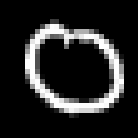
\includegraphics[width=0.14\linewidth]{fig/input_108.png} &
    
\includegraphics[width=0.14\linewidth]{fig/input_777.png} \\
    番号 1 & 番号 4 & 番号 100 & 番号 108 & 番号 777 \\
    正解 0 & 正解 9 & 正解 5 & 正解 0 & 正解 8 \\
    出力 9 & 出力 9 & 出力 9 & 出力 6 & 出力 9 \\
  \end{tabular}
  \caption{入力した画像と、その正解ラベルおよびプログラムの出力}
  \label{fig:input1}
\end{figure}

5回のうち、正解したのは画像番号 4 の1回のみであった。
この画像の正解ラベルはたまたま 9 であり、プログラムはほとんどの入力に対して 9 を出力するため、偶然一致したにすぎない。
画像番号 1 と 108 はどちらも正解ラベルが 0 の画像であるが、出力は 9 と 6 で異なっており、同じ数字を入力しても同じ出力になるとは限らない。
学習を行っていないため、重みはランダムな値であり、認識結果は正解ラベルとは無関係な値となる。
なお、画像番号 1～1000 のうち 9 以外を出力したのは画像番号 108 の1枚のみであった（\ref{sec:k1cmp}節の表\ref{tab:k1cmp}）。

%% -------------------------------------------------------------
\subsection{リファクタリング}
\label{sec:ref1}
%% -------------------------------------------------------------
まず動作するプログラムを作成し（リファクタリング前）、その後コードを見直して改善した（リファクタリング後）。

リファクタリングとは、本来「プログラムの外部から見た振る舞いを変えずに、内部の構造を改善すること」を指すが、
今回の見直しでは、構造の改善に加えて、計算結果が変わる数値計算上の修正も同時に行った。
そのため以下では、コードの修正を「構造の改善（振る舞いを変えない）」と「振る舞いを変える改善」に分けて示す。

リファクタリングの方針を決めるにあたっては、生成AIである Claude（Anthropic 社の Opus 5.5 モデル）に元のプログラムの改善点を質問した。
また、得られた提案をそのまま採用するのではなく、インターネット上の解説記事で考え方と手法について調べ、それぞれの変更の意味とプログラムの構造を理解したうえで適用した。
参考にした文献の一覧を付録\ref{sec:refs}に示す。


課題1で行ったリファクタリングを表\ref{tab:ref1}にまとめる。

\begin{table}[H]
  \centering
  \caption{課題1で行ったリファクタリング}
  \label{tab:ref1}
  \small
  \begin{tabular}{L{0.22\linewidth}L{0.36\linewidth}L{0.33\linewidth}}
    \toprule
    手法 & 変更内容 & 目的・効果 \\
    \midrule
    \multicolumn{3}{l}{\textbf{構造の改善（振る舞いを変えない）}} \\
    変数名の変更 & \texttt{var} を \texttt{std1}、\texttt{std2} に変更 & 中身は分散ではなく標準偏差であり、名前と意味を一致させる \\
    不要なコードの削除 & 中間結果を表示するデバッグ用の \texttt{print} を5行削除 & 出力を認識結果のみにし、読みやすくする \\
    コメントの追加 & \texttt{number\_of\_images} などにコメントを追加 & 変数の意味を明確にする \\
    \midrule
    \multicolumn{3}{l}{\textbf{振る舞いを変える改善}} \\
    入力の正規化と定数化 & 画素値を \texttt{pixel\_value}（$=255$）で割り、$[0,1]$ にする & 中間層への入力が大きくなりすぎてシグモイド関数が 0 や 1 に張り付く（飽和する）のを防ぐ \\
    重み初期化の修正 & 標準偏差を層ごとに $1/\sqrt{784}$、$1/\sqrt{500}$ とする & その層への入力ノード数 $N$ に応じた $1/\sqrt{N}$ にする \\
    オーバーフロー対策 & シグモイド関数の入力を \texttt{np.clip} で $[-500, 500]$ に制限 & \texttt{np.exp} のオーバーフローを防ぐ \\
    \bottomrule
  \end{tabular}
\end{table}

主な変更箇所の前後を以下に示す。

\begin{lstlisting}[style=before, caption={【前】重みの初期化と入力の前処理}, label=lst:k1b]
var = 1.0 / np.sqrt(image_pixels) #重みの初期化に使う分散

W1 = var * np.random.randn(image_pixels, hidden_nodes)  #入力層から隠れ層への重み
W2 = var * np.random.randn(hidden_nodes, class_size)  #隠れ層から出力層への重み

def input_layer(input_data):
    ...
    return (X[input_data].reshape(-1))
\end{lstlisting}

\begin{lstlisting}[style=after, caption={【後】重みの初期化と入力の前処理}, label=lst:k1a]
std1 = 1.0 / np.sqrt(image_pixels) #入力層→隠れ層の重みの初期化に使う標準偏差
std2 = 1.0 / np.sqrt(hidden_nodes) #隠れ層→出力層の重みの初期化に使う標準偏差

W1 = std1 * np.random.randn(image_pixels, hidden_nodes)  #入力層から隠れ層への重み
W2 = std2 * np.random.randn(hidden_nodes, class_size)  #隠れ層から出力層への重み

def input_layer(input_data):
    ...
    return X[input_data].reshape(-1).astype(np.float64) / pixel_value #画素値を0〜1に正規化
\end{lstlisting}

\subsubsection{変更前後の比較}
\label{sec:k1cmp}
リファクタリング前後のプログラムに、画像番号 1～1000 の1000枚をそれぞれ入力し、出力を比較した。
また、どの変更が結果に影響したかを調べるため、リファクタリング後のプログラムから「振る舞いを変える改善」を1つずつ元に戻した版も実行した。
シード値はすべて 81 にそろえた。

元のプログラムは画像番号をキーボードから1つずつ受け取るため、1000枚を試すには1000回実行する必要がある。
そこで、検証用のプログラム \texttt{verification/kadai1\_compare.py} を別に作成した。
元のプログラムは、シード値を 81 に固定したうえで乱数を生成しているため、入力する画像番号によらず毎回同じ重みとなる。
検証用のプログラムでは、これと同じ手順で重みを1回だけ作り、画像番号 1～1000 の画像を行列にまとめて一度に順伝播を計算した。
各版の違い（正規化の有無、標準偏差を層ごとに変えるか、\texttt{np.clip} の有無）は引数で切り替えられるようにした。
そして、各版について次の3つを求めた。
\begin{itemize}
  \item \textbf{正解率}：出力されたクラスが MNIST の正解ラベルと一致した画像の割合。
  \item \textbf{飽和率}：1000枚分の中間層の出力（シグモイド関数の値、$1000 \times 500$ 個）のうち、0.01 未満または 0.99 より大きいものの割合。
  \item \textbf{出力されたクラスの内訳}：各クラスが出力された回数を数え、多い順に並べたもの。
\end{itemize}
また、まとめて計算した結果が元のプログラムを1枚ずつ実行した結果と同じであることを確かめるため、リファクタリング前後の元のプログラムに画像番号 1、100、500、1000 を実際に入力し、出力が一致することを確認した。
結果を表\ref{tab:k1cmp}に示す。

\begin{table}[H]
  \centering
  \caption{課題1のリファクタリング前後の比較（画像1000枚）}
  \label{tab:k1cmp}
  \small
  \begin{tabular}{lccl}
    \toprule
    プログラム & 正解率 & 飽和率 & 出力されたクラスの内訳 \\
    \midrule
    前                       & 9.2\%  & 95.5\% & 9：721、6：213、4：43、3：12、1：8、7：3 \\
    後                       & 10.0\% & 0.0\%  & 9：999、6：1 \\
    後（正規化なし）         & 9.2\%  & 95.5\% & 前と同じ \\
    後（標準偏差を層で共通） & 10.0\% & 0.0\%  & 後と同じ \\
    後（\texttt{np.clip} なし） & 10.0\% & 0.0\%  & 後と同じ \\
    \bottomrule
  \end{tabular}
\end{table}

この結果から、以下のことが分かる。
\begin{itemize}
  \item \textbf{正規化によって結果が変わっている}：正規化だけを元に戻すと、正解率、飽和率、クラスの内訳がすべて前と同じになった。
  \item \textbf{正規化によりシグモイド関数の飽和が解消された}：前は中間層の出力の 95.5\% が 0 か 1 に張り付いていたが、後は 0\% になった。画素値（最大 255）のままでは全結合層の出力の絶対値が大きくなりすぎるためである。
  \item \textbf{標準偏差の修正と \texttt{np.clip} によるクラス内訳への影響は少ない}：標準偏差の修正では、出力確率の値は変わったが、予測クラスは変わらなかった。また今回の入力では \texttt{np.exp} がオーバーフローするほど大きな値は現れず、\texttt{np.clip} は結果に影響しなかった。念のため、\texttt{np.clip} は、極端な入力に備える安全対策として残している。
\end{itemize}

なお、正解率はどちらも約 10\% であり、10クラスからでたらめに選んだ場合と同程度である。
これは学習を行っていないためであり、リファクタリングの前後で認識性能に差はない。

%% -------------------------------------------------------------
\subsection{工夫点}
%% -------------------------------------------------------------
\begin{itemize}
  \item \textbf{定数の名前付け}：画像サイズ、画素値の最大値、クラス数、中間層のノード数などを意味のある名前の変数として定義し、可読性と保守性を高めた。
  \item \textbf{画素値の正規化}：画素値を 255 で割って $[0, 1]$ に正規化し、シグモイド関数の飽和を防いだ（表\ref{tab:k1cmp}）。
  \item \textbf{オーバーフロー対策}：シグモイド関数では \texttt{np.clip} により入力を制限し、ソフトマックス関数では最大値を引いてから \texttt{np.exp} を計算することで、指数関数のオーバーフローを防いだ。
  \item \textbf{段階的なリファクタリング}：まず動作するプログラムを作り、その後に見直す手順をとった。Git でそれぞれの段階をコミットし、変更前後を比較できるようにした。また、変更を1つずつ元に戻した版と比べることで、どの変更が結果に影響したかを確かめた。
\end{itemize}

%% -------------------------------------------------------------
\subsection{問題点}
%% -------------------------------------------------------------
\begin{itemize}
  \item 学習を行っていないため、入力に関わらずほぼ常に 9 が出力される（1000枚中999枚）。乱数で初期化した重みの偏りによるものである（表\ref{tab:k1cmp}）。
  \item MNIST データのファイルパスを絶対パスで記述しているため、別の環境では書き換えが必要である。また、関数を呼ぶたびにデータセット全体を読み込んでおり、効率が悪い。これらは課題2のリファクタリングで解消した（表\ref{tab:ref2}）。
\end{itemize}


%% =============================================================
\section{課題2：ミニバッチ対応とクロスエントロピー誤差}
%% =============================================================

\subsection{課題内容}
課題1のプログラムを、ミニバッチ（＝複数枚の画像）を入力可能とするように改良し、さらにクロスエントロピー誤差を計算するプログラムを作成する。

\subsection{ネットワークの構成}
バッチサイズを $B$ とし、$B$ 枚の画像を行方向に並べた行列 $X \in \mathbb{R}^{B \times 784}$ を入力とする。
各層の計算は行列積でまとめて行う。
\begin{align}
  Y_1 &= \sigma\!\left(X W_1 + \bm{b}_1^{\top}\right) \in \mathbb{R}^{B \times M} \\
  Y_2 &= \mathrm{softmax}\!\left(Y_1 W_2 + \bm{b}_2^{\top}\right) \in \mathbb{R}^{B \times C}
\end{align}
ソフトマックス関数は各行（各画像）ごとに独立して適用する。

正解ラベルを one-hot ベクトル $\bm{t}_i \in \{0,1\}^{C}$ で表すと、ミニバッチに対するクロスエントロピー誤差の平均は次式で与えられる。
\begin{equation}
  E = \frac{1}{B}\sum_{i=1}^{B}\sum_{k=1}^{C} -t_{i,k}\log y_{2,ik}
\end{equation}

\subsection{作成したプログラムの説明}
課題1からの変更点を中心に説明する。

\begin{enumerate}
  \item 学習データ 60000 枚から $B = 100$ 枚をランダムに（重複なく）選択する。
  \item 正解ラベルを one-hot ベクトルに変換する。
  \item 順伝播を行列演算で一括計算する。
  \item クロスエントロピー誤差の平均を計算して出力する。
\end{enumerate}

主要な関数を表\ref{tab:func2}に示す（リファクタリング後）。
\begin{table}[H]
  \centering
  \caption{課題2で作成した主な関数}
  \label{tab:func2}
  \begin{tabular}{ll}
    \toprule
    関数名 & 役割 \\
    \midrule
    \texttt{load\_mnist}    & MNIST の画像とラベルを読み込む \\
    \texttt{get\_minibatch} & ミニバッチの選択、正規化、one-hot 変換 \\
    \texttt{dense\_layer}   & 全結合層の計算 \\
    \texttt{sigmoid}        & シグモイド関数 \\
    \texttt{softmax}        & ソフトマックス関数（行ごと） \\
    \texttt{cross\_entropy} & クロスエントロピー誤差（バッチ平均） \\
    \texttt{forward}        & 順伝播をまとめて行う \\
    \texttt{main}           & 重みの初期化から誤差の出力までの実行部分 \\
    \bottomrule
  \end{tabular}
\end{table}

\begin{lstlisting}[caption={ミニバッチの取得とone-hotベクトルへの変換}, label=lst:batch]
def get_minibatch(X, Y, batch_size):
    #ランダムに選んだbatch_size枚の画像(正規化済み)と正解ラベル(one-hot)を返す
    selected_indices = np.random.choice(X.shape[0], batch_size, replace=False) #ランダムな画像を選ぶ
    x = X[selected_indices].reshape(batch_size, -1).astype(np.float64) / pixel_value #画素値を0〜1に正規化
    y = np.eye(class_size)[Y[selected_indices]] #one-hotベクトルに変換
    return x, y
\end{lstlisting}

\begin{lstlisting}[caption={ミニバッチ対応のソフトマックス関数とクロスエントロピー誤差}, label=lst:ce]
def softmax(x):
    exp_x = np.exp(x - np.max(x, axis=-1, keepdims=True)) #np.expのオーバーフローを防ぐ
    return exp_x / np.sum(exp_x, axis=-1, keepdims=True)

def cross_entropy(y_true, y_pred):
    eps = 1e-7 #log(0)を防ぐ
    return -np.sum(y_true * np.log(y_pred + eps)) / y_pred.shape[0] #バッチ内の平均
\end{lstlisting}

\subsection{実行結果}
リファクタリング後のプログラム（シード値 0、バッチサイズ 100）の実行結果を以下に示す。

\begin{lstlisting}[language={}, numbers=none, caption={課題2の実行例}, label=lst:run2]
> python layers.py
2.4589022144299957
\end{lstlisting}

学習前の重みでは各クラスの出力がほぼ均等になると考えられるため、誤差は $\log 10 \approx 2.30$ 付近の値になると予想される。
実際の誤差は 2.46（シード値 0）、2.67（シード値 10）であり、予想した $\log 10 \approx 2.30$ に近い値となった。
予想よりやや大きいのは、ランダムな重みによって出力が完全には均等にならず、正解とは異なるクラスに確率が偏るためと考えられる。

%% -------------------------------------------------------------
\subsection{リファクタリング}
\label{sec:ref2}
%% -------------------------------------------------------------
課題1と同様に、まず動作するプログラムを作成し、その後コードを見直して改善した。
変更は課題1と同じく「構造の改善（振る舞いを変えない）」と「振る舞いを変える改善」に分けて示す。


課題2で行った変更を表\ref{tab:ref2}にまとめる。

\begin{table}[H]
  \centering
  \caption{課題2で行った変更}
  \label{tab:ref2}
  \small
  \begin{tabular}{L{0.22\linewidth}L{0.36\linewidth}L{0.33\linewidth}}
    \toprule
    手法 & 変更内容 & 目的・効果 \\
    \midrule
    \multicolumn{3}{l}{\textbf{構造の改善（振る舞いを変えない）}} \\
    関数の分割 & \texttt{input\_layer} を、データを読み込む \texttt{load\_mnist} と、ミニバッチを選ぶ \texttt{get\_minibatch} に分割 & 6万枚の読み込みが1回で済むようにし、効率的に何度もバッチを読み出せるようにする \\
    関数の抽出 & 順伝播の処理を \texttt{forward} 関数にまとめる & 学習や評価の際に繰り返し呼び出せる \\
    グローバル変数への依存の除去 & \texttt{cross\_entropy} で割る値を、グローバル変数 \texttt{batch\_size} から \texttt{y\_pred.shape[0]} に変更 & 関数が外部の変数に依存せず、どのバッチサイズでも正しく平均をとれる \\
    式の簡略化 & 二重の \texttt{np.sum} を1つにまとめる & 同じ計算をより読みやすく書く \\
    変数のスコープの縮小 & 重み \texttt{W1} などをグローバル変数から \texttt{main} 内のローカル変数にし、引数で渡す & 意図しない書き換えを防ぎ、データの流れを明確にする \\
    エントリポイントの導入 & 実行部分を \texttt{main} 関数にまとめ、\texttt{if \_\_name\_\_ == "\_\_main\_\_":} から呼ぶ & 他のファイルから import しただけでは計算が実行されない \\
    ハードコードの除去 & 絶対パスを \texttt{pathlib} によるスクリプト基準の相対パスに変更 & 別の環境やディレクトリでもそのまま動く \\
    パラメータ化 & \texttt{load\_mnist(kind)} で学習用、テスト用を切り替え可能にする & テストデータの読み込みにも同じ関数を使えるようにする。 \\
    説明用変数の導入 & 長い \texttt{return} 文を \texttt{x}、\texttt{y} に分けて返す & 何を返しているかが分かりやすくなる \\
    不要なコードの削除 & 未使用の \texttt{matplotlib}、\texttt{number\_of\_images}、コメントアウトした行、不要な行継続の \texttt{\textbackslash} を削除 & コードの簡潔化\\
    コメントの追加 & 各関数の先頭に、処理内容と入出力を説明するコメントを追加 & 関数の入出力を明確にする \\
    \midrule
    \multicolumn{3}{l}{\textbf{振る舞いを変える改善}} \\
    数値安定化 & \texttt{np.log} の中に小さな値 \texttt{eps}（$=10^{-7}$）を足す & 予測確率が 0 のときの $\log 0 = -\infty$ や \texttt{nan} を防ぐ \\
    \bottomrule
  \end{tabular}
\end{table}

また、乱数を使う順番（$W_1 \to W_2 \to \bm{b}_1 \to \bm{b}_2 \to$ ミニバッチの選択）はリファクタリング前と同じにした。
これにより、同じシード値を与えればリファクタリングの前後で同じ結果が得られ、振る舞いが変わっていないことを確認できる。

実際に、シード値をそろえてリファクタリング前後のプログラムを実行し、クロスエントロピー誤差を比較した。
結果を表\ref{tab:seedcmp}に示す。
ここで「後（$\mathit{eps}=0$）」は、振る舞いを変える改善である \texttt{eps} を一時的に 0 にして実行した結果である。

\begin{table}[H]
  \centering
  \caption{シード値をそろえたときのリファクタリング前後の誤差}
  \label{tab:seedcmp}
  \small
  \begin{tabular}{rlll}
    \toprule
    シード値 & 前 & 後 & 後（$\mathit{eps}=0$） \\
    \midrule
    0  & 2.4589035261042866 & 2.4589022144299957 & 2.4589035261042866 \\
    10 & 2.6671179625628105 & 2.6671161841438570 & 2.6671179625628105 \\
    \bottomrule
  \end{tabular}
\end{table}

リファクタリング後の誤差は前と比べて $10^{-6}$ 程度小さくなった。
これは \texttt{np.log} の中に $\mathit{eps}=10^{-7}$ を足したことによる差である。
実際に \texttt{eps} を 0 にすると、どちらのシード値でも前後の結果が浮動小数点数の全桁まで一致した。
したがって、\texttt{eps} 以外の変更（関数の分割、\texttt{forward} の抽出、\texttt{main} 関数の導入など）はプログラムの振る舞いを変えておらず、リファクタリングとして正しく行えていることが確認できた。
また、\texttt{eps} による差は誤差の値に比べて十分小さく、計算結果への影響は無視できると考える。

主な変更箇所の前後を以下に示す。

\begin{lstlisting}[style=before, caption={【前】データの読み込みとミニバッチの選択が1つの関数に混在}, label=lst:k2b1]
def input_layer(batch_size):
    X = mnist.download_and_parse_mnist_file(\
    r"C:\caex4\le4nn\le4nn\mnist_data\train\train-images-idx3-ubyte.gz")
    Y = mnist.download_and_parse_mnist_file(\
    r"C:\caex4\le4nn\le4nn\mnist_data\train\train-labels-idx1-ubyte.gz")

    selected_indices = np.random.choice(X.shape[0], batch_size, replace=False) #ランダムな画像を選ぶ

    return X[selected_indices].reshape(batch_size, -1).astype(np.float64) / pixel_value,\
            np.eye(class_size)[Y[selected_indices]] #one-hotベクトルに変換
\end{lstlisting}

\begin{lstlisting}[style=after, caption={【後】読み込みとミニバッチの選択を別の関数に分割}, label=lst:k2a1]
DATA_DIR = Path(__file__).parent / "mnist_data" #MNISTデータの置き場所

def load_mnist(kind="train"):
    #MNISTの画像とラベルを読み込む (kindは"train"か"test")
    prefix = "train" if kind == "train" else "t10k"
    X = mnist.download_and_parse_mnist_file(str(DATA_DIR / kind / f"{prefix}-images-idx3-ubyte.gz"))
    Y = mnist.download_and_parse_mnist_file(str(DATA_DIR / kind / f"{prefix}-labels-idx1-ubyte.gz"))
    return X, Y

def get_minibatch(X, Y, batch_size):
    #ランダムに選んだbatch_size枚の画像(正規化済み)と正解ラベル(one-hot)を返す
    selected_indices = np.random.choice(X.shape[0], batch_size, replace=False) #ランダムな画像を選ぶ
    x = X[selected_indices].reshape(batch_size, -1).astype(np.float64) / pixel_value #画素値を0〜1に正規化
    y = np.eye(class_size)[Y[selected_indices]] #one-hotベクトルに変換
    return x, y
\end{lstlisting}

\begin{lstlisting}[style=before, caption={【前】グローバル変数に依存したクロスエントロピー誤差}, label=lst:k2b2]
def cross_entropy(y_true, y_pred):
    return np.sum(-np.sum(y_true * np.log(y_pred), axis=-1, keepdims=True)) / batch_size
\end{lstlisting}

\begin{lstlisting}[style=after, caption={【後】入力から枚数を求め、log(0)を防ぐ}, label=lst:k2a2]
def cross_entropy(y_true, y_pred):
    eps = 1e-7 #log(0)を防ぐ
    return -np.sum(y_true * np.log(y_pred + eps)) / y_pred.shape[0] #バッチ内の平均
\end{lstlisting}

\begin{lstlisting}[style=before, caption={【前】実行部分がファイルの最上位に書かれている}, label=lst:k2b3]
vectorized_input, vectorized_labels = input_layer(batch_size)
hidden_layer_output = dense_layer(vectorized_input, W1, b1)
hidden_layer_activation = sigmoid(hidden_layer_output)
output_layer_output = dense_layer(hidden_layer_activation, W2, b2)
output_layer_activation = softmax(output_layer_output)
#final_output = np.argmax(output_layer_activation)
cross_entropy_loss = cross_entropy(vectorized_labels, output_layer_activation)

print(cross_entropy_loss)
\end{lstlisting}

\begin{lstlisting}[style=after, caption={【後】順伝播を関数化し、実行部分をmain関数にまとめる}, label=lst:k2a3]
def forward(x, W1, b1, W2, b2):
    #順伝播を行い、各クラスの確率 (バッチ数, class_size) を返す
    hidden_layer_activation = sigmoid(dense_layer(x, W1, b1))
    return softmax(dense_layer(hidden_layer_activation, W2, b2))

def main():
    ... # 重みの初期化（省略）
    X, Y = load_mnist("train")
    x_batch, y_batch = get_minibatch(X, Y, batch_size)

    y_pred = forward(x_batch, W1, b1, W2, b2)
    print(cross_entropy(y_batch, y_pred))

if __name__ == "__main__":
    main()
\end{lstlisting}

%% -------------------------------------------------------------
\subsection{工夫点}
%% -------------------------------------------------------------
\begin{itemize}
  \item \textbf{行ごとのソフトマックスを適用}：\texttt{axis=-1, keepdims=True} を指定して各行の和をとることで、ミニバッチの各画像に独立してソフトマックス関数を適用できるようにした。
  \item \textbf{one-hot ベクトルの生成}：単位行列 \texttt{np.eye(10)} の特定の行を取り出すことで、 one-hot ベクトルへ変換した。
  \item \textbf{リファクタリング前後の検証}：乱数を使う順番を変えずにリファクタリングし、シード値をそろえて前後の誤差を比較することで、振る舞いが変わっていないことを確かめた（表\ref{tab:seedcmp}）。
\end{itemize}

%% -------------------------------------------------------------
\subsection{問題点}
%% -------------------------------------------------------------
\begin{itemize}
  \item 重みとバイアスは乱数で初期化しただけの、学習していないでたらめな値であるため、出力される確率は正解ラベルに集中しない。そのため、クロスエントロピー誤差は 0 に近づくことはなく、実際の値も 2.46（シード値 0）と、10クラスに均等な確率を出力した場合の $\log 10 \approx 2.30$ 程度の大きな値にとどまる。誤差を小さくするには、誤差逆伝播法などで重みを学習する必要がある。
\end{itemize}


%% =============================================================
\section{おわりに}
%% =============================================================
本レポートでは、MNIST の手書き数字画像を入力とする3層ニューラルネットワークを作成した。
課題1では、画像1枚を入力として 0～9 のいずれかを出力する推論のプログラムを作成し、課題2では、それをミニバッチに対応させたうえで、クロスエントロピー誤差を計算できるようにした。
また、どちらの課題でも、まず動作するプログラムを作ってからリファクタリングを行い、変更の前後で結果を比較して、それぞれの変更がプログラムの振る舞いにどう影響するかを確かめた。

深層学習の仕組みそのものは以前から知っていたが、実際に自分で行列の計算を組み立て、画像を入力して数字が出力されるところまで動かしてみると、数式で見ていたものがそのままプログラムとして動くことに改めて感動した。

リファクタリングについては、作成した直後は、動いているのだからこのコードで十分だと考えていた。
しかし、インターネットで調べたり AI に改善点を質問したりする中で、変数名の付け方や関数の分け方、正規化や数値計算上の工夫など、より良くできる点が多くあることを知った。
特に課題2では、今後の課題で学習や評価を行うことを見据えて、データの読み込み、ミニバッチの取り出し、順伝播をそれぞれ関数に分けて整理した。

現時点では学習を行っていないため、認識結果はでたらめな値しか出ず、正解率も約 10\% にとどまっているのは残念である。
今後の課題で誤差逆伝播法による学習を実装し、認識精度がどこまで向上するのかを確かめるのが楽しみである。

%% =============================================================
\appendix
\section{ソースコード}
%% =============================================================
提出したソースファイルの一覧を表\ref{tab:files}に示す。
\begin{table}[H]
  \centering
  \caption{提出ファイル}
  \label{tab:files}
  \begin{tabular}{ll}
    \toprule
    ファイル名 & 内容 \\
    \midrule
    \texttt{kadai1\_before.py} & 課題1（リファクタリング前） \\
    \texttt{kadai1\_after.py}  & 課題1（リファクタリング後） \\
    \texttt{kadai2\_before.py} & 課題2（リファクタリング前） \\
    \texttt{kadai2\_after.py}  & 課題2（リファクタリング後） \\
    \bottomrule
  \end{tabular}
\end{table}

%% 方法A：Overleaf の src/ フォルダにアップロードした .py を読み込む
%%        （.py を差し替えればレポートにも自動で反映される）
%%        前後のコードが不要なら、その行を % でコメントアウトする
\inputcode{style=before, caption={課題1のプログラム（リファクタリング前）}, label=lst:k1before}{src/kadai1_before.py}
\inputcode{style=after,  caption={課題1のプログラム（リファクタリング後）}, label=lst:k1after}{src/kadai1_after.py}
\inputcode{style=before, caption={課題2のプログラム（リファクタリング前）}, label=lst:k2before}{src/kadai2_before.py}
\inputcode{style=after,  caption={課題2のプログラム（リファクタリング後）}, label=lst:k2after}{src/kadai2_after.py}

%% 方法B：直接貼り付ける場合は以下のように書く
% \begin{lstlisting}[caption={課題1のプログラム全体}, label=lst:task1]
% ここに Python コードを貼り付け
% \end{lstlisting}

%% =============================================================
\section{参考文献}
\label{sec:refs}
%% =============================================================
リファクタリングの方針を決める際に参考にした文献を以下に示す（Web ページの参照日はすべて 2026年10月9日）。

%% thebibliography が自動で出す見出し（\section*{参考文献}）は使わず、上の付録の見出しを使う
\begingroup
\renewcommand{\section}[2]{}
\raggedright %URL の前で文字間が空きすぎるのを防ぐ
\begin{thebibliography}{9}
  
  \bibitem{pymain}
    Python Software Foundation: 「\texttt{\_\_main\_\_} --- トップレベルのコード環境」、Python ドキュメント、
    \url{https://docs.python.org/ja/3/library/__main__.html}
    \newline（\texttt{main} 関数と \texttt{if \_\_name\_\_ == "\_\_main\_\_":} の使い方）
  \bibitem{pypathlib}
    Python Software Foundation: 「\texttt{pathlib} --- オブジェクト指向のファイルシステムパス」、Python ドキュメント、
    \url{https://docs.python.org/ja/3/library/pathlib.html}
    \newline（スクリプトの場所を基準にした相対パスの書き方）
  \bibitem{keionorm}
    「Keras/TensorflowでMNISTデータセットの画像分類」、
    \newline\url{https://www.ailab.ics.keio.ac.jp/b4_induction_training/docs/dl/mnist_notebook.html}
    \newline（MNIST の画素値を 255 で割り、0～1 に正規化する前処理）
  \bibitem{sigclip}
    @segavvy：「ゼロから作るDeep Learningで素人がつまずいたことメモ:3章」、Qiita、2019。
    \url{https://qiita.com/segavvy/items/6d79d0c3b4367869f4ea}
    \newline（シグモイド関数の入力を \texttt{np.clip} で制限し、\texttt{np.exp} のオーバーフローを防ぐ方法）
  \bibitem{crossent}
    @yamaken\_1130：「ニューラルネットワークの基礎を整理しよう(2) ー前回の補足」、Qiita、2021。
    \url{https://qiita.com/yamaken_1130/items/8aaee2b2ec08289fe44a}
    \newline（one-hot 表現と、$\log 0$ を防ぐために微小な値 $10^{-7}$ を足すクロスエントロピー誤差の実装）
\end{thebibliography}
\endgroup

\end{document}
